\documentclass[letterpaper,twocolumn,10pt]{article}
\usepackage{epsfig,xspace,url}
\usepackage{authblk}

\usepackage{graphicx}
\graphicspath{ {./images/} }

\usepackage{listings}
\lstset{
basicstyle=\small\ttfamily,
columns=flexible,
breaklines=true
}

\usepackage[
backend=biber,
style=alphabetic,
sorting=ynt
]{biblatex}

\addbibresource{references.bib}

\title{Thread Network In Clyde Building Report}
\author{Devon Ward, Daniel Harman}

\begin{document}

\maketitle

\subsection*{Introduction}

Thread is a mesh networking protocol which has been developed mainly for smart home devices \cite*{thread_website}. The main idea is to remove a single point of failure for the networking smart home devices, allowing them to communicate with each other and avoid having a potential problem where one device fails, taking down the entire network. Another beneficial aspect of thread is that it is designed to be low power \cite*{Thread_paper_1}, which is also a really good thing for IoT devices, which are often power constrained. 

One problem that Thread networks have currently is that they are not very well tested. There are many sources that have successfully tested Thread networks and proven that they can operate in a noisy environment but most publications are focused on throughput achievements, rather than distance and reliability.  

Our project seeks to attempt to classify the performance of Thread in the Clyde engineering building at Brigham Young University, and determine if a Thread network is capable of allowing two users to communicate from the graduate research lab in CB 480 to anywhere in the Clyde building. In doing so, we also seek to understand how many nodes are required to allow for uninterrupted communication in the Clyde building. 

Our experiments seek to quantify the range of the Thread devices using ESPRESSIF ESP32-H2 Dev boards \cite*{ESP32_h_board} to get an estimate of how many routers we will require for the Thread network. We then plan to strategically place the routers throughout the Clyde building, and attempt to walk through the building without losing connection to the parent node in the graduate lab. We will quantify exactly how many router Thread nodes we will require, and attempt to use the minimum number possible.

We found that we only required one Thread router node, one parent node, and one child node to allow the child node to go all around the basement of the Clyde, and through the rest of the building without losing connection. We were also able to briefly go outside the Clyde building and still communicate with the graduate lab. 

\subsection*{Related Work}

There are many sources that have successfully tested Thread networks and proven that they can operate in a noisy environment \cite*{Thread_noisy_env} but very little to classify their performance in indoor urban environments. Work has previously been done to quantify the throughput of Thread networks in an indoor area \cite*{Thread_on_drones} \cite*{Thread_lightbulb} but most publications are focused on throughput achievements, rather than distance and reliability.

Many tutorials exist for building a Thread network with an ESP32 \cite*{Thread_tutorial} as well as details on how to implement the design and program the microcontroller \cite*{Thread_tutorial_2} to run the thread network.  

There are papers that discuss distance as a metric for the Thread network operating \cite*{Thread_wheelchair} that talk about the jitter in the network. However, they do not discuss the maximum distance for transmission when the Thread mesh breaks down. For our project we wanted to investigate the maximum transmission distance for an indoor environment containing lots of metal doors over multiple floors, something that is not present in the current literature. 

\subsection*{Methodology}

We approached our problem in the following steps: 
\begin{enumerate}
    \item Program the ESP32-h to run a thread network
    \item Set up a TCP thread connection built on top of UDP to allow secure reliable communication over the thread network to measure performance
    \item Measure distance leader and child thread devices can communicate
    \item Add router thread nodes until we can map the entire Clyde building
\end{enumerate}

In order to program the ESP32-h devices, we used ESPRESSIF's tutorials which allow us to flash the ESP32 devices with an already functional thread network. This significantly reduced the time for development of the thread network. 

Second, we wanted to set up a TCP connection. This is unintuitive because thread by design uses UDP, and there is no real sense of acknowledgements, since the mesh network is utilizing router devices to send UDP packets from the leader to the child nodes. However, we want to see when we lose connection with the child nodes as we walk around in the Clyde building. Therefore, we use a TCP client built on top of the UDP client to see when we stop receiving acknowledgement packets from the child to the leader node. 

Once the TCP mesh network is set up and running, we then walk around the Clyde building with only the leader and child, and categorize the number of walls we can transmit through, and the standard distance we can communicate. By doing this we can find the blind spots of the Clyde building that we cannot reach without router nodes in the mesh network. Then we add single router nodes one at a time and see how many router nodes we need to cover all of our previously identified blind spots and have reliable communication throughout the entire Clyde building. 

\subsection*{Implementation/Experimentation}

% Describe your experiments and your results. Discuss your results.
\subsection{Programming ESP32h2 Module}

The ESP32h2 module is a relatively new chip from Espressif, meaning that support for it has not made it to the larger space of IDE's, such as Arduino or VScode's extension Platform.io. Thus, we installed the VScode Espressif IDF extension, which is developed and supported by Espressif as direct access to their software development kit (SDK). The extension conveniently has access to each of their tutorials \cite*{Thread_tutorial_2}. We used the tutorial "ot\_cli", or OpenThread Command Line Interface. The program allows an instance of OpenThread, an open source implementation of the Thread standard to be run via a command line interface with the ESP32 using a serial port connection. Opening the project in VScode via the Espressif IDF extension allows you to 
\begin{enumerate}
    \item Select a connected USB device/port
    \item Build the example project
    \item Flash the ESP32
\end{enumerate}

\begin{figure}
    \centering
    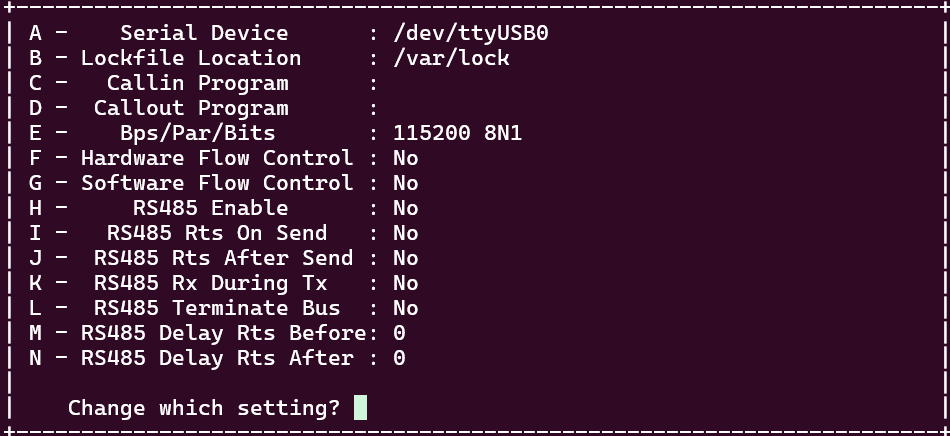
\includegraphics[width=0.75\linewidth]{Figures/minicom_screenshot.png}
    \caption{Screenshot of the Minicom Settings}
    \label{fig:minicom}
\end{figure}

\subsection{Setting up the Thread Network}

Once flashed, a serial connection needs to be established with the ESP32 to setup the thread network and send messages. We used the Minicom serial port terminal emulator for Linux, with settings as displayed in \ref{fig:minicom}. Once connected, we ran the following to setup a Thread network for the network leader. A network leader is a role within a Thread mesh, that provides a key used to join the network and as well as assuming some necessary centralized functions for the network. To set up the network, we ran:
\begin{lstlisting}
> factoryreset
> dataset init new
> dataset commit active
> ifconfig up
> thread start 
> state
> ipaddr
> dataset active -x
\end{lstlisting}

The last two commands are how the IPv6 address for the leader and the Thread network key are found respectively. These need to be copied over for the other devices to use to join the network and to setup a TCP socket with the leader for testing purposes.

For the child devices (those on the network, but not the leader), we connected to the network using:

\begin{lstlisting}
> factory reset
> dataset set active $PUT THREAD KEY HERE$
> ipconfig up
> thread start
> state
\end{lstlisting}

Note the state is just a test to establish connection to the network and status within the network.

\subsection{Setting up the TCP connection}

For the server side, we used the following:
\begin{lstlisting}
> tcpsockserver open
> tcpsockserver bind :: 12345
> tcpsockserver send MESSAGE_WITH_NO_SPACES
\end{lstlisting}
and for the client side we connect to the open socket by using:
\begin{lstlisting}
> tcpsockclient open
> tcpsockclient connect $PUT IPV6 ADDR HERE$ 12345
> tcpsockclient send $MESSAGE_WITH_NO_SPACES$
\end{lstlisting}

\subsection{Experiment}

The experiment that we ran involved running 3 Thread devices to determine the maximum length of connectivity that the mesh could support. The leader was in the ECEn graduate student lab as a stationary device. The other two were connected to laptops and moved throughout the Clyde Engineering building. The path taken is shown in Fig. \ref{fig:clyde}. Connection to the leader was strong through out the 4th, 3rd and most of the 2nd floor. The connection began to break down when entering the basement, but strategic placement of the intermediate node allowed the client to get TCP packet through. Even intermittent service outside was possible. 

\begin{figure}[h]
    \centering
    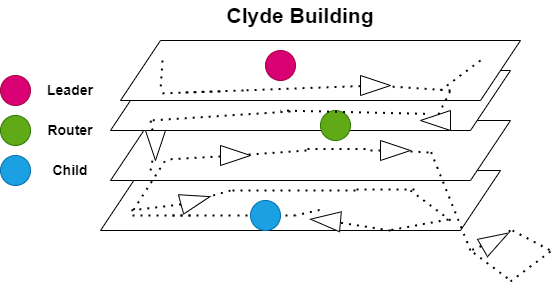
\includegraphics[width=0.75\linewidth]{Figures/Clyde_Map.png}
    \caption{Map of Experiment Path Taken}
    \label{fig:clyde}
\end{figure}

Fig. \ref{fig:mesh_setup} shows the output of the mesh following a successful setup. Once a device is on the network, there is no way to determine if it acting as a mesh router. This posses the issue of knowing whether or not the placement of an intermediate device is actually beneficial or not. This is helped though by messages that appear on the intermediate device when it fails to pass-along a message, shown in Fig. \ref{fig:mesh_error}.

\begin{figure}
    \centering
    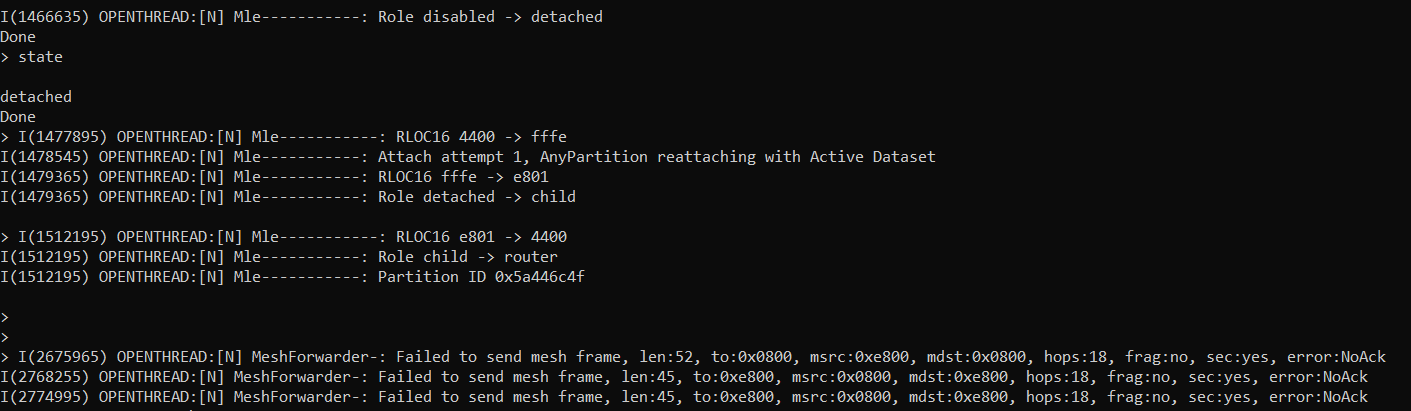
\includegraphics[width=0.75\linewidth]{Figures/Mesh_Error_Response.png}
    \caption{Command Line Mesh Error Response}
    \label{fig:mesh_error}
\end{figure}

\begin{figure}
    \centering
    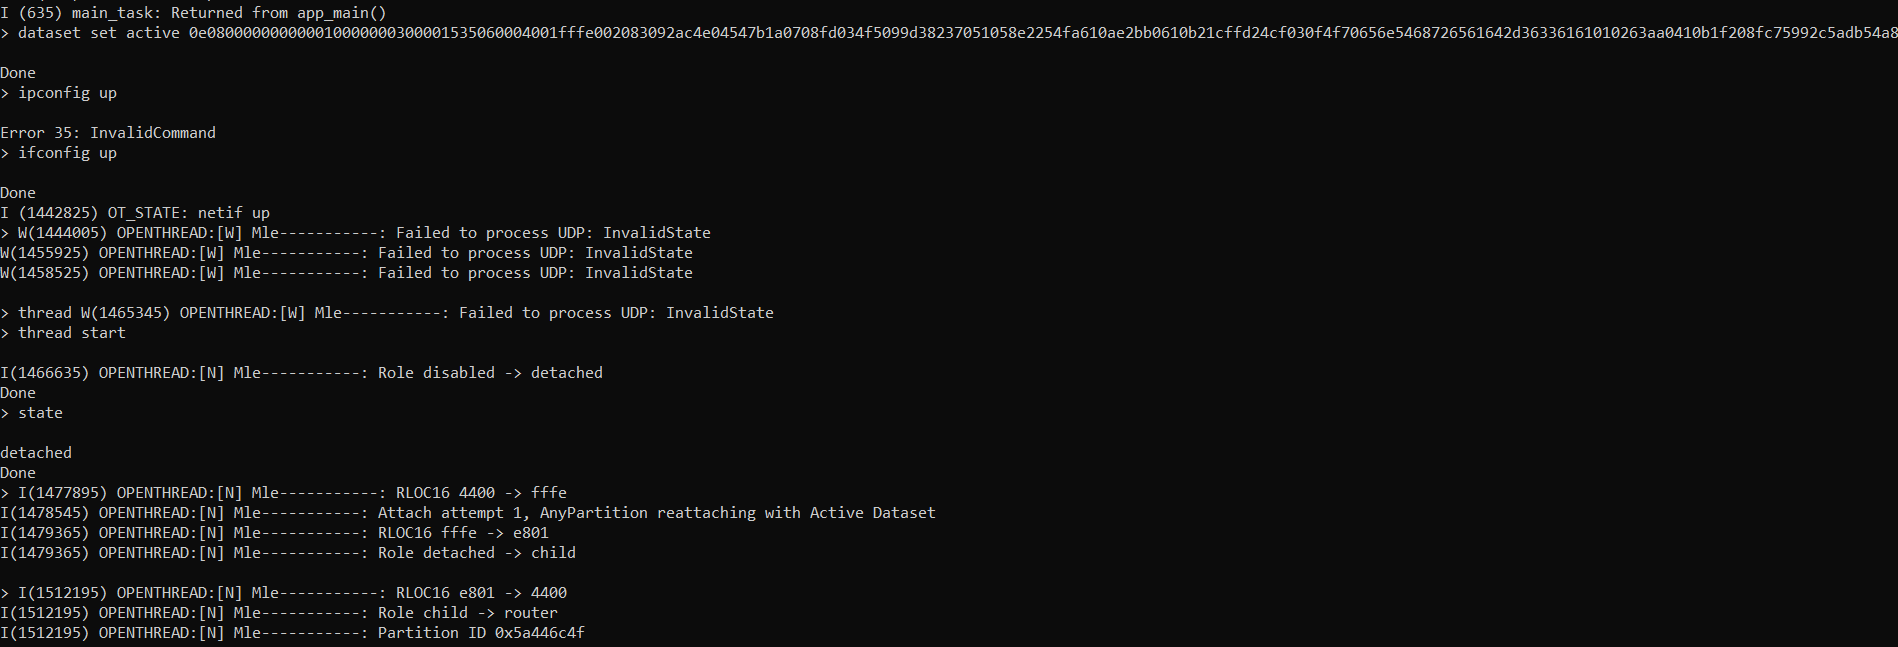
\includegraphics[width=0.75\linewidth]{Figures/Mesh_Initial_Setup.png}
    \caption{Command Line Mesh Setup Output}
    \label{fig:mesh_setup}
\end{figure}

To determine if the 3rd device actually played a significant role, we shut it down for a time and re-walked many of the same areas in the basement and the 1st floor of the Clyde building. The connection between leader and child was essentially the same except for specific spots in the basement, meaning that there really wasn't a significant advantage introduced by the intermediate device, which is unfortunate for Thread, but demonstrates the robustness of Zigbee.

\subsection*{Conclusion}

Thread is an interesting protocol with potential for many applications. It does not however offer much in terms of the meshing, over direct connections between Zigbee devices. The software support and marketing of these devices will need to increase though before they can reach their full realization and improvements.

\printbibliography

\end{document}